\documentclass[11pt,a4paper]{article}

\usepackage[T1]{fontenc}
\usepackage[utf8]{inputenc}
\usepackage[a4paper,margin=1in]{geometry}
\usepackage{hyperref}
\usepackage{graphicx}
\usepackage{booktabs}
\usepackage{enumitem}
\usepackage{xcolor}
\usepackage{float}

\title{Monitize Case Report\\\large Embodied AI with LeRobot and SmolVLA}
\author{Taylan Dursun}
\date{\today}

\begin{document}

\maketitle
\tableofcontents
\newpage

\section{Overview}
This report documents the current progress for the Monitize case study.
At this stage, the focus is on \textbf{Task 1} and \textbf{Task 2}.
\textbf{Task 3} is intentionally excluded and will be added in a later revision.

\section{Task 1: Embodied AI Exploration with SmolVLA and LeRobot}

\subsection{Objective}
The objective is to run a pretrained SmolVLA policy in simulation and evaluate whether the robot behavior is coherent for the selected robot-task setup.

\subsection{Part A: Research and Concept}

\subsubsection{LeRobot}

LeRobot is an open-source robot learning framework developed by Hugging Face. It is built on top of PyTorch and provides tools for working with robot datasets, pretrained policies, fine-tuning workflows, and real-world robot control interfaces \cite{lerobot_github}.

The main goal of LeRobot is to make robotics and Physical AI more accessible. Instead of requiring every researcher or developer to build separate tools for data collection, dataset storage, model training, and deployment, LeRobot provides a more unified ecosystem.

One important part of this ecosystem is \texttt{LeRobotDataset}. It enables large robotics datasets to be stored, shared, streamed, and visualized in a standardized format through the Hugging Face Hub. This is important because modern robot learning methods depend heavily on large and well-structured datasets.

Compared to traditional robotics control stacks, LeRobot focuses more on data-driven policy learning. In a classical robotics pipeline, engineers usually design separate modules for perception, motion planning, inverse kinematics, trajectory generation, and low-level control. In LeRobot, the focus is on collecting robot demonstrations, training or fine-tuning policies, and deploying learned policies through a standardized interface. However, LeRobot does not completely replace classical robotics components. Low-level control, calibration, safety limits, and hardware communication are still necessary in real robotic systems. This difference is illustrated in Figure~\ref{fig:lerobot-vs-traditional}.

\begin{figure}[H]
\centering
\small

\textbf{Traditional robotics control stack}
\vspace{0.2cm}

\fbox{
\parbox{0.9\textwidth}{
\centering
Sensor Data
$\rightarrow$
State Estimation
$\rightarrow$
Motion Planning
$\rightarrow$
Inverse Kinematics
$\rightarrow$
Trajectory Generation
$\rightarrow$
Low-Level Control
$\rightarrow$
Robot Actuation
}
}

\vspace{0.5cm}

\textbf{LeRobot / data-driven robot learning workflow}
\vspace{0.2cm}

\fbox{
\parbox{0.9\textwidth}{
\centering
Robot Demonstrations / Dataset
$\rightarrow$
Policy Training or Fine-Tuning
$\rightarrow$
Learned Policy
$\rightarrow$
Standardized Robot Interface
$\rightarrow$
Robot Action
}
}

\caption{Comparison between a traditional robotics control stack and the LeRobot-oriented data-driven workflow.}
\label{fig:lerobot-vs-traditional}
\end{figure}

\subsubsection{SmolVLA}

SmolVLA is a compact Vision-Language-Action model developed by Hugging Face for robotics applications \cite{smolvla_docs}. A VLA model takes visual observations, natural language instructions, and robot state information as input, then outputs robot actions.

The main motivation behind SmolVLA is efficiency. Large VLA models can require expensive hardware and high computational resources. SmolVLA is designed to make VLA-based robotics more accessible to researchers, developers, and hobbyists using consumer-level hardware \cite{smolvla_blog}.

Architecturally, SmolVLA combines a vision-language model with an action expert. The vision-language part processes images and language instructions, while the action expert generates robot actions. In simple terms, the first part helps the model understand the scene and the task, and the second part decides how the robot should move.

SmolVLA also supports asynchronous inference. This means that action prediction and action execution can be separated. While the robot is executing one chunk of actions, the model can predict the next action chunk. This can help make robot behavior smoother and more responsive.

\subsubsection{Difference Between VLA Models, LLMs, and Vision Models}

A standard Large Language Model mainly processes and generates text. For example, it can answer questions, summarize documents, or write explanations. A vision model mainly processes images and produces visual outputs such as object labels, image features, bounding boxes, or segmentation masks.

A Vision-Language-Action model is different because it connects perception and language understanding to physical robot actions. In a robotics context, the input is not only text or image data, but also the current state of the robot. The output is not a text answer or an image label, but an action that can be executed by the robot.

This can be summarized as:

\[
\text{Visual Observation} + \text{Language Instruction} + \text{Robot State}
\rightarrow
\text{Robot Action}
\]

For this reason, VLA models are especially relevant for embodied AI. They allow a robot to interpret a scene, understand a task described in natural language, and generate actions to complete that task.

\subsection{Part B: Simulation and Inference}

\subsubsection{Model Selection}
\begin{table}[h]
\centering
\begin{tabular}{ll}
\toprule
Item & Value \\
\midrule
Checkpoint name & \texttt{lerobot/smolvla\_libero} \\
Hugging Face URL & \url{https://huggingface.co/lerobot/smolvla_libero} \\
Trained dataset & \texttt{lerobot/libero} \\
Robot arm in training set & Panda \\
Why this checkpoint (not base) & Fine-tuned checkpoint aligned with LIBERO tasks and Panda embodiment \\
\bottomrule
\end{tabular}
\caption{Selected SmolVLA checkpoint details}
\end{table}

The selected checkpoint was \texttt{lerobot/smolvla\_libero}. This model is a fine-tuned SmolVLA policy rather than a base checkpoint, which makes it more appropriate for direct evaluation. The associated dataset metadata for \texttt{lerobot/libero} indicates that the robot type is \texttt{panda}. This was an important selection criterion, because using a checkpoint trained on a different embodiment would likely produce inconsistent or incoherent actions.

\subsubsection{Simulation Setup}
The simulation pipeline combined two complementary components. First, I used the LIBERO benchmark environment, because the selected SmolVLA checkpoint was trained for LIBERO-style tasks. Second, I separately validated Panda simulation setup using the MuJoCo Menagerie Panda model to confirm that the underlying robot embodiment and MuJoCo rendering pipeline were functioning correctly.

For robot validation, I used the Franka Emika Panda assets from MuJoCo Menagerie under the Panda scene configuration. The Panda simulation opened correctly in MuJoCo, and the robot joints could be manipulated interactively through the viewer. This provided a useful sanity check before running policy inference.

For policy evaluation, I used the LIBERO environment through LeRobot with the \texttt{libero\_10} task suite. The observation configuration included two RGB camera streams (agent view and wrist view) together with robot state features such as joint positions, joint velocities, gripper states, and end-effector pose features. This setup matched the expected multimodal input structure of the selected SmolVLA checkpoint.

Robot-model compatibility was checked at two levels. First, the checkpoint-dataset pairing showed that the policy was fine-tuned on LIBERO using a Panda robot. Second, the runtime environment used Panda-based LIBERO tasks, which preserved embodiment consistency between the training data and evaluation environment.

\subsubsection{Inference Procedure}
The inference procedure was implemented through \texttt{lerobot-eval}. The overall process was as follows:

\begin{enumerate}[leftmargin=1.5em]
	\item The LIBERO environment was initialized with \texttt{env.type=libero} and \texttt{env.task=libero\_10}.
	\item The SmolVLA checkpoint \texttt{lerobot/smolvla\_libero} was loaded through \texttt{policy.pretrained\_path}.
	\item Observations were collected from the RGB camera streams and robot state tensors, then mapped into the feature structure expected by LeRobot and SmolVLA.
	\item The policy generated robot actions autoregressively during evaluation, and those actions were executed in the environment.
	\item Videos were automatically recorded by the evaluation pipeline for each task and stored in the evaluation output directory.
\end{enumerate}

In practice, several rollout lengths were tested. Very short rollouts initially produced videos shorter than one second, which made it difficult to judge behavior quality. After increasing the rollout horizon to approximately 5 and 10 seconds, the policy behavior became much easier to observe. Because the available GPU memory was limited to 4 GB, full evaluation on GPU led to out-of-memory errors during policy loading. As a result, the final evaluation was executed on CPU, which was slower but stable.

\subsubsection{Results and Evaluation}
The main positive result is that the full evaluation pipeline worked end-to-end: the environment initialized successfully, the policy loaded correctly, rollouts were executed, and evaluation videos were generated. This confirms that the selected SmolVLA checkpoint could be integrated with LeRobot and a Panda-compatible LIBERO simulation workflow.

Behaviorally, the policy did not solve every scenario in an ideal way, but the motions were generally coherent. In longer rollouts, the robot produced meaningful task-related movement patterns rather than random or unstable actions. In particular, some trials showed that the robot could interact with the bottles and throw them toward the basket area, which indicates that the policy captured non-trivial task structure.

There were also important limitations. First, short rollout horizons were misleading, because they made the policy appear inactive or ineffective when in reality the video duration was simply too small to observe the behavior. Second, GPU evaluation was limited by memory capacity, so stable testing had to be performed on CPU. Third, the aggregated success metrics for the initial short evaluation remained low, which suggests that task completion quality is sensitive to rollout horizon, evaluation settings, and computational constraints.

Overall, I consider the result successful for this case study. The objective of Part B was to run a pretrained SmolVLA policy in simulation and observe coherent robot behavior. That objective was achieved. Although the performance was not perfect and not every task was solved cleanly, the system produced interpretable, embodiment-consistent, and task-relevant motions.

\paragraph{Qualitative Rollout Frames}
Representative frames from two evaluation videos are shown below.

\begin{figure}[h]
	\centering
	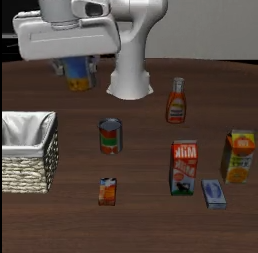
\includegraphics[width=0.48\linewidth]{figures/task1_rollout_frame_1.png}
	\hfill
	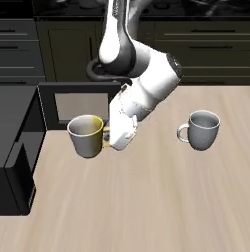
\includegraphics[width=0.48\linewidth]{figures/task1_rollout_frame_2.png}
	\caption{Qualitative rollout snapshots from two LIBERO evaluation videos. The left frame corresponds to Episode 1 and the right frame corresponds to Episode 10. These examples illustrate that, although the policy does not solve every scenario perfectly, it produces coherent task-related motion.}
\end{figure}

\subsection{Task 1 Deliverables Checklist}
\begin{itemize}[leftmargin=1.5em]
	\item One-page research and implementation summary.
	\item Model choice with robot compatibility justification.
	\item Inference evaluation (successes, failures, reasons).
	\item Rendered Task 1 video or GIF generated from LIBERO evaluation outputs.
\end{itemize}

\newpage
\section{Task 2: Vision-Based Teleoperation (Hand to Robot)}

\subsection{Objective}
The objective is to extract human hand motion from video and map that motion to the Trossen VX300s right arm in simulation using inverse kinematics. The target movement is a bottle lifting and pouring trajectory.

\subsection{Task Definition}
This task connects three components: visual hand tracking, motion mapping, and robot control. A video of a human hand provides the source motion. From this video, the hand or wrist trajectory must be estimated in 3D. That trajectory is then converted into an end-effector target for the VX300s robot arm. Finally, an inverse kinematics solver computes the robot joint values required to reproduce the lifting and pouring behavior in MuJoCo.

\subsection{Planned Pipeline}
The intended implementation pipeline is:

\begin{enumerate}[leftmargin=1.5em]
	\item Validate the VX300s simulation model in MuJoCo.
	\item Select a hand-video source for the pouring motion.
	\item Extract hand landmarks using MediaPipe Hand Landmarker or MANO.
	\item Isolate the wrist trajectory and relevant orientation cues.
	\item Map the human hand motion to robot end-effector targets.
	\item Solve robot joint configurations with inverse kinematics.
	\item Replay the motion in simulation and render a side-by-side comparison video.
\end{enumerate}

\subsection{Robot Setup}
The robot model used for Task 2 was the Trossen VX300s right arm from MuJoCo Menagerie. The simulation scene was loaded from the Menagerie-provided \texttt{scene.xml} file, and a headless smoke test confirmed that the model could be initialized and stepped successfully in MuJoCo. An interactive viewer run also confirmed that the robot could be visualized and manipulated in simulation.

The VX300s model exposes 8 configuration variables and 7 actuators, which is consistent with a 6-DoF arm plus gripper actuation. For motion replay, the \texttt{pinch} site at the gripper was treated as the operational end-effector point. This made it possible to map the human hand motion to a physically meaningful target point on the robot.

\subsection{Vision Input and Landmark Extraction}
The input video was a custom first-person recording named \texttt{pouring.mp4}. In the video, the hand performs a bottle-lifting and pouring gesture, although no physical bottle is visible. This is still sufficient for prototyping, because the main motion cues needed for the task are wrist translation, elevation, and tilt.

For landmark extraction, I used MediaPipe Hand Landmarker. The implementation was adapted to the MediaPipe Tasks API, since the installed MediaPipe package exposed the modern \texttt{tasks} interface rather than the older \texttt{solutions} interface. The extraction pipeline produced two outputs: an annotated video showing the detected hand landmarks, and a JSON file containing the frame-by-frame landmark coordinates.

The landmark detection was stable enough for downstream processing. The wrist point and the MCP joints of the index, middle, and pinky fingers were consistently detected, which provided enough information to estimate both a wrist trajectory and coarse hand orientation cues. This was an important result, because Task 2 does not need full dexterous hand reconstruction at this stage; it mainly needs a reliable control signal for the robot arm.

\subsection{Motion Mapping and IK Strategy}
The motion transfer pipeline was implemented in three stages. First, the landmark JSON was reduced to a wrist trajectory representation. Besides the wrist position itself, the pipeline also computed orientation-related features such as palm-axis direction, palm normal, and a simple pouring angle derived from the wrist-to-middle-finger direction. These signals were then smoothed with a moving average filter to reduce frame-to-frame jitter.

Second, the smoothed wrist motion was mapped into the VX300s workspace. The initial version used direct min-max normalization, but this produced only a rough approximation of the gesture. A better result was achieved by using \textbf{relative motion mapping}: the first detected wrist pose was treated as a reference, and subsequent wrist displacements were converted into robot end-effector displacements around a predefined workspace center. This made the replay feel more like motion transfer rather than absolute coordinate matching.

Third, a simple numerical inverse kinematics routine was used to move the robot end-effector toward the target positions. The \texttt{pinch} site was used as the controlled point, and the solver updated the arm joints using a damped Jacobian pseudoinverse method. Wrist rotation was controlled separately using the pouring-angle signal and a palm-axis yaw component. This strategy is still approximate, but it was sufficient to obtain coherent lifting and tilting behavior.

\subsection{Results and Evaluation}
The main evaluation criterion for Task 2 was qualitative coherence rather than exact kinematic imitation. I compared the reference hand video and the robot replay by checking three behaviors: whether the robot lifts in the same general phase as the hand, whether the wrist tilt resembles a pouring gesture, and whether the timing feels natural.

The initial replay already produced non-random motion, but the gesture did not closely resemble the original hand action. After adding orientation-aware features and switching to relative mapping, the replay quality improved significantly. In particular, the robot could reproduce a wrist rotation similar to the approximately 90-degree pouring motion seen in the video. The motion speed was initially too fast, but adjusting replay timing with a playback speed of \texttt{0.85} made the robot behavior better aligned with the reference video.

At the current stage, the result is not a perfect imitation, but it is a convincing and technically meaningful prototype. The robot motion is not identical to the hand motion, yet it is coherent, task-related, and clearly closer to the intended pouring behavior than a random or unstable baseline.

The final Task 2 artifacts include the annotated hand-landmark video, the processed wrist trajectory files, the mapped VX300s target trajectory, a replay video of the robot motion, and a side-by-side comparison video between the source hand motion and the robot replay. These outputs are sufficient to demonstrate that the full perception-to-control pipeline is working.

\subsection{Task 2 Deliverables Checklist}
\begin{itemize}[leftmargin=1.5em]
	\item Hand landmark extraction pipeline with annotated output video.
	\item VX300s motion replay in MuJoCo.
	\item Side-by-side comparison video between the input hand motion and robot replay.
	\item Short technical evaluation of motion quality, timing, and current limitations.
\end{itemize}

\section{Reproducibility Notes}
\begin{itemize}[leftmargin=1.5em]
	\item Environment files: \texttt{environment.yml}, \texttt{environment\_full.yml}, \texttt{requirements\_lock.txt}
	\item OS: Linux.
	\item GPU: NVIDIA GeForce RTX 3050 Laptop GPU with 4 GB VRAM.
	\item Final stable evaluation used CPU because GPU loading of the policy caused out-of-memory errors.
	\item Known limitations: dependency compatibility issues between modern MuJoCo packages and older LIBERO/robosuite expectations required environment adjustment; rollout quality was sensitive to episode length.
	\item Future steps: improve orientation-aware control, replace the simple IK approximation with a more constrained end-effector controller, and refine motion timing and scaling for closer imitation quality.
\end{itemize}

\bibliographystyle{plain}
\bibliography{references}

\end{document}
